\documentclass[11pt]{article}

\usepackage[letterpaper,margin=0.75in]{geometry}
\usepackage{booktabs}
\usepackage{graphicx}
\usepackage{listings}
\usepackage{fixltx2e}
\usepackage{verbatim}
\usepackage{color}

\definecolor{dkgreen}{rgb}{0,0.6,0}
\definecolor{gray}{rgb}{0.5,0.5,0.5}
\definecolor{mauve}{rgb}{0.58,0,0.82}
\definecolor{orange}{RGB}{255,119,0}
\definecolor{purple2}{RGB}{153,0,153}

\setlength{\parindent}{1.4em}

\begin{document}

\lstset{
  language=Python,
  basicstyle=\small\ttfamily, % print whole listing small
  keywordstyle=\color{orange},
  keywordstyle={[2]\color{purple2}},
  identifierstyle=,           % nothing happens
  commentstyle=\color{dkgreen},% green comments
  stringstyle=\ttfamily\color{mauve},      % typewriter type for strings
  showstringspaces=false,     % no special string spaces
  numbers=left,
  numberstyle=\tiny\color{gray},
  numbersep=5pt,
  frame=tb,
}

\title{CS460 Lab 1 Report: Network Simulation}

\author{Michael K. Eagar}

\date{January 24th, 2014}

\maketitle

\section{Two Nodes}

I set up the two node network in the simulator by first creating the two nodes, n\textsubscript{1} and n\textsubscript{2}. I then created the bidirectional link between them (using two unidirectional links in the simulator, $n_{1}\to{n_{2}}$ and $n_{2}\to{n_{1}}$).
\\
\noindent
For the first scenario, the bidirectional link was created with bandwidth of 1 Mbps, and a propagation delay of 1 second:
\lstinputlisting[breaklines = true, firstline = 21, lastline = 34, caption = Two Nodes Scenario 1]{./twonodes/twoNodes1.py}

\noindent
Program output: 1.008 1 0 1.008 0.008 1.0 0\\
According to the simulation the total amount of time it took to send one 1000 byte packet from node 1 to node 2 was 1.008 sec.\\
The calculations below show the simulator to be correct:\\
$\indent L = 8,000\ bits \\
\indent R = 1,000,000\ bps \\
\indent d_{prop} = 1\ sec \\
\indent d_{trans} = \frac{L}{R} = \frac{8,000\ bits}{1,000,000\ bps} = 0.008\ sec \\
\indent d_{total} = d_{prop} + d_{trans} = 1\ sec + 0.008\ sec = 1.008\ sec$
\\
\vspace{0.25cm}

\noindent
In the second scenario, the bandwidth was reduced to 100 bps with a propagation delay of 10 ms:
\lstinputlisting[breaklines = true, firstline = 21, lastline = 34, caption = Two Nodes Scenario 2]{./twonodes/twoNodes2.py}

\noindent
Program output: 80.01 1 0 80.01 80.0 0.01 0\\
According to the simulation for this scenario, the total time taken to send one 1000 byte packet from node 1 to node 2 was 80.01 sec.\\
The calculations below show the simulator to be correct:\\
$\indent L = 8,000\ bits \\
\indent R = 100\ bps \\
\indent d_{prop} = 10ms = 0.01\ sec \\
\indent d_{trans} = \frac{L}{R} = \frac{8,000\ bits}{100\ bps} = 80\ sec \\
\indent d_{total} = d_{prop} + d_{trans} = 80\ sec + 0.01\ sec = 80.01\ sec$
\\
\vspace{0.25cm}

\noindent
For the third scenario, the bandwidth was increased back to 1 Mbps, but the propagation delay was kept at 10 ms:
\lstinputlisting[breaklines = true, firstline = 21, lastline = 34, caption = Two Nodes Scenario 3]{./twonodes/twoNodes3.py}

\noindent
Program output: \\
\indent0.018 1 0 0.018 0.008 0.01 0 \\
\indent0.026 2 0 0.026 0.008 0.01 0.008\\
\indent0.034 3 0 0.034 0.008 0.01 0.016\\
\indent2.018 4 2.0 0.018 0.008 0.01 0.0\\
\\
\noindent
The simulator shows that it takes one 1000 byte packet 0.018 sec to travel from node 1 to node 2 along this link.\\
The calculations below show this to be correct:\\
$\indent L = 8,000\ bits \\
\indent R = 1,000,000\ bps \\
\indent d_{prop} = 10ms = 0.01\ sec \\
\indent d_{trans} = \frac{L}{R} = \frac{8,000\ bits}{1,000,000\ bps} = 0.008\ sec \\
\indent d_{total} = d_{prop} + d_{trans} = 0.008\ sec + 0.01\ sec = 0.018\ sec\\$
\\
From the output we can see that the 1\textsuperscript{st} and 4\textsuperscript{th} packets have no queuing delay (the last number on their respective lines) while packets \textsuperscript{\#}2 and \textsuperscript{\#}3 have queuing delay of 0.008 sec and 0.016 sec respectively. These two accumulate the delay because packets 1 through 3 are all sent at $time = 0\ sec$, so \textsuperscript{\#}2 has to wait for packet \textsuperscript{\#}1 to transmit, and \textsuperscript{\#}3 for both \textsuperscript{\#}1 and \textsuperscript{\#}2 to transmit completely. Packet \textsuperscript{\#}4 doesn't get sent until $time = 2.0\ sec$, so there are no other packets in queue or being transmitted, and it is transmitted right away.\\
\\
Total time for each packet is: \textsuperscript{\#}1 - 0.018 sec, \textsuperscript{\#}2 - 0.026 sec, \textsuperscript{\#}3 - 0.034 sec, \textsuperscript{\#}4 - 2.018 sec\\

\section{Three Nodes}

\textbf{Scenario 1 - Two Fast Links}\\
\noindent
To set up this three node network in the simulator, I first created the three nodes: n\textsubscript{1}, n\textsubscript{2}, and n\textsubscript{3}. I then set up the fast 1 Mbps links connecting the three nodes. I created the links as follows: $n_{1}\to{n_{2}}$, $n_{2}\to{n_{1}}$, $n_{2}\to{n_{3}}$, and $n_{3}\to{n_{2}}$. Each link has a propagation delay of 100 ms.\\

\lstinputlisting[breaklines = true, firstline = 21, lastline = 46, caption = Three Nodes Scenario 1a]{./threenodes/threeNodes1a.py}

\noindent
\textbf{Part A}\\
\textit{Node A transmits a stream of 1 kB packets to node C. How long does it take to transfer a 1 MB file, divided into 1 kB packets, from A to C? Which type of delay dominates?}\\
\indent It will take 8.208 sec to fully transfer a 1 MB file divided into 1,000 1 KB packets from node A to node C. Transmission delay accounts for 8.008 sec of the time taken to transfer the file, while propagation delay only accounts for 0.2 sec. Therefore, transmission delay ($d_{trans}$) dominates. This matches the output of the simulator (see below), thus proving the simulator correct.\\
\\
\noindent
\textbf{Part B}\\
Network setup for part B is the same as for part A, except that the links' bandwidths were changed to 1 Gbps. Propagation delays remained at 100 ms.
\lstinputlisting[breaklines = true, firstline = 26, lastline = 26, caption = Three Nodes Scenario 1b]{./threenodes/threeNodes1b.py}
\textit{If both links are upgraded to a rate of 1 Gbps, how long does it take to transfer a 1 MB file from A to C?}\\
\indent If both links are upgraded to a rate of 1 Gbps then it will only take 0.208008 sec to transfer a 1 MB file from node A to node C.\\

\vspace{0.25cm}
\noindent
\textbf{Scenario 2 - One Fast and One Slow Link}\\
\noindent
To set up the second three node network, I created the three nodes just like before, but when setting up the links between the nodes I created them as follows.\\
\indent Fast links (1 Mbps, 100ms $d_{prop}$): $n_{1}\to{n_{2}}$ and $n_{2}\to{n_{1}}$\\
\indent Slow links (256 Kbps, 100ms $d_{prop}$): $n_{2}\to{n_{3}}$, and $n_{3}\to{n_{2}}$\\
The links between node B and node C have had their bandwidth reduced to 256 Kbps, but the propagation delay remains the same.\\

\lstinputlisting[breaklines = true, firstline = 21, lastline = 46, caption = Three Nodes Scenario 2]{./threenodes/threeNodes2.py}
\textit{Node A transmits 1000 packets, each of size 1 kB, to node C. How long would it does it take to transfer a 1 MB file, divided into 1 kB packets, from A to C?}
\indent It would take 31.458 sec to transfer a 1 MB file divided into one thousand 1 kB packets from node A to node C. In order to ensure that there was no queuing delay at node A in the simulation for this network, I created each packet to be sent at successively later times (the transmission delay for the link from A to B multiplied by the packet \#).  This caused the only queuing delay in the system to occur at node B.\\
\\
Below is the output from the simulator for Scenario 2. I know it is correct because of the calculations involving the last packet of the file. The 1000\textsuperscript{th} packet is transmitted at 7.992 sec($t_{trans}$). Transmission time at node A is 8 ms (or 0.008 seconds), and at node B is 31.25 ms (or 0.03125 sec) for a total transmission delay of 0.03925 seconds ($d_{trans}$). $d_{prop} = 0.2\ sec$ total for both links, and the last packet's queuing delay at node B is 23.22675 sec. For the last packet, $t_{trans} + d_{trans} + d_{prop} + d_{queue} = Time_{trans}$ for the entire file. This works out as follows:
$$t_{trans} + d_{trans} + d_{prop} + d_{queue} = 7.992\ sec + 0.03925\ sec + 0.2\ sec + 23.22675\ sec = 31.458\ sec$$ total transmission time for a 1 MB file.\\
\lstinputlisting[breaklines = true, firstline = 0, caption = Three Nodes Scenario 2 output]{./threenodes/threeNodes2.out}

\section{Queuing Delay}
\noindent
\textbf{Experiment Setup}\\
\indent Below is the basic code I used to generate the data for this experiment. In order to generate varying loads, I changed the value of the \textit{load\_scale} variable on line 53, running the experiment with loads from 0.1 to 0.9, increasing in increments of 0.1, as well as at loads of 0.95 and 0.98. I set the duration for the load to 30 seconds in order to collect a larger amount of data in order to give a better estimate for my averages for queuing delay.
\\
For each load, the script generated a large number of 1 kB packets and simulated transmitting them along a 1 Mbps link. The packets had randomly generated start times, and because of the large amount generated, queuing delay at the transmitting node was ensured. In order to collect the data from the simulation, I redirected \textit{stdout} to a file when running the python script for each load level. These are saved in the textit{queuingtheory} directory as queing10.out through queuing98.out.\\\\
\noindent
\textbf{Queuing Delay Code}
\lstinputlisting[breaklines = true, firstline = 0, caption = queuingdelay.py]{./queuingtheory/queuingdelay.py}

\vspace{1.0cm}
\noindent
\textbf{Queuing Delay Plots}
\\
As can be seen in the plots below, the simulation data matched the theoretical values of queuing delay quite well. It only really starts to deviate from the theory at the highest load values, near 95 and 98 percent loads. I think this small amount of difference could even be eliminated by increasing the duration of the simulation and collecting additional data.
\\
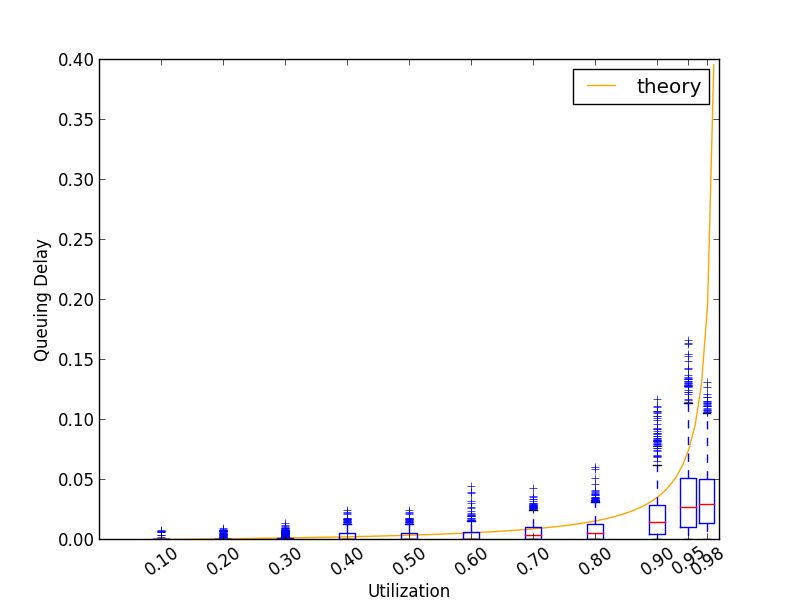
\includegraphics[width=15cm]{queuingtheory/QueuingDelayBoxplot}\\
\vspace{1.0cm}
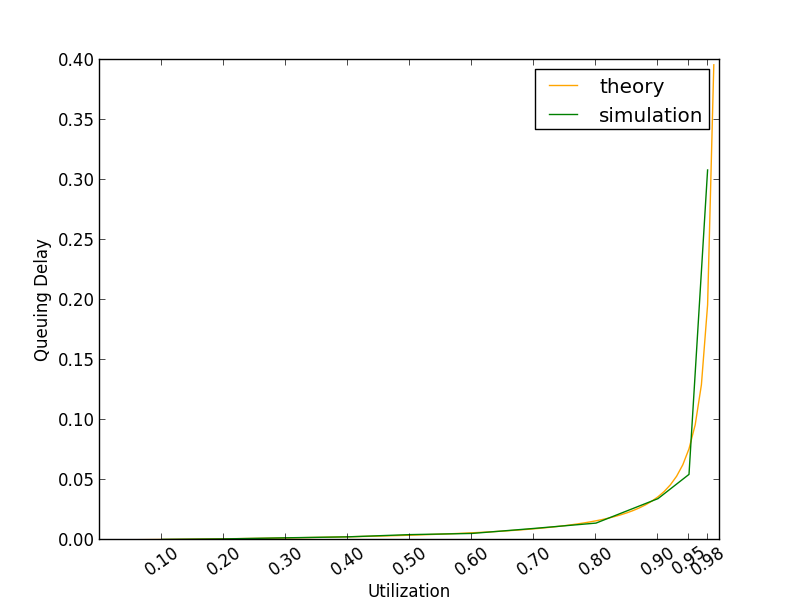
\includegraphics[width=15cm]{queuingtheory/QueuingDelayAverages}

\end{document}
